\chapter{Discussion}
\label{chap:discussion}

The results you have collected and the process you went through to develop the project have been presented earlier.  This Chapter is used to talk about your interpretations of results or the process.  It might be a discussion of the language you used.  A tool that you started to use but then stopped using for some reason.  It could give insight into the evolution of your process.

\section{Development decisions}
\subsection{Using scriptable objects in the project}
    - Discuss scriptable objects, pros and cons. 
    - Cite Unity talk.
    - Used for modifiers and shop items
    
\subsection{Moving from Confluence to ShareLaTeX for writing the thesis}
    - Originally wanted to write thesis in confluence as we kept our meeting notes there and having a centralised documentation/thesis hub would be nice. After taking a deeper look at ShareLaTeX and the thesis template we ended up deciding to move over from confluence to ShareLaTeX. We still write our meeting notes on confluence before transferring it over though.
    - Thesis looks more professional, easier to do things like citations and direct PDF output is very convenient. 

\subsection{Moving from virtual functions to interfaces for the Ability base class}
    - Issue with having to create new versions of ServerCallback() per new type of parameter we wanted to send. 
    - Luckily we can use interfaces to somewhat alleviate this problem. 
    - Abilities needing to use server callbacks can implement different versions of IServerCallback. IServerCallback has several versions where templated parameters can be put into its functions.  
    - Still needs to create a new command in docking per new type of parameter, but we are able to avoid doing the same for Ability when using the interface, reducing a fair share of code bloat. 

\subsection{Providing ergonomic controls when using a twin stick scheme}
    - Needed to provide ergonomic and fast access to the most frequently used buttons. 
    - In a twin stick scheme, both thumbs are used for the sticks. Leaves the shoulder and trigger buttons accessible by other fingers. This is why we stick with four abilities, one for each shoulder button and trigger.
    - Less important buttons like the shop, dock/undock etc buttons could then be mapped to ABXY. 

\subsection{Whether to move from Unity3D to Unity2D after the release of Unity 5.6}
    - Originally started with Unity3D in the case we wanted navmesh functionality for pathfinding if we got that far during development. 
    - Unity 5.6 now supports navmeshes in 2D as well.
    - Would generally be a big benefit for network bandwidth as we would save one float for each synchronised Vector3. Rigidbodies contain a lot of these so it would be a significant improve in network performance. 
    
    - Other parts like raycasting and so on would also be cheaper. 
    - Unity 5.6 launched very late into the development cycle so moving over to it would take too many resources that should better be spent on the thesis. 

\subsection{Potentially using the player's field of view as a means of visibility checking instead of ray casting}
One idea that we thought of while developing was to use the field of view component for visibility checking rather than regular ray casting. This would allow abilities like the flash grenade in the brawler kit to only stun players who had the grenade in their field of view at the time of explosion rather than using a ray cast + dot product. We ultimately decided against implementing this due to a few reasons. 

The first reason is that the field of view is fairly computationally expensive. The component uses many ray casts to generate a mesh that we use as a visibility mask for the players. It would not be possible to directly synchronise the generated meshes so we would have to synchronise the various variables for the component itself and reconstruct the field of view on the server. Doing so would allow us to have a player local field of view for the sake of responsiveness while using the server's version for any visibility checking. This could work if the server was ran as a dedicated server, but our project is primarily focused on trying to create a MOBA using peer to peer connectivity so a implementation like this would not be very effective as it would place a lot of extra load on the host player. 

A server authoritative visibility check like this would be far better for security reasons compared to local checking, but we currently have a middle ground where the server uses ray casts and dot products to check player face directions. This is independent of the field of view component so we have less control in regards to limiting the view angles and so on.

Another issue is that keeping the field of view synchronised would take a fair share of additional bandwidth if we want the server to keep itself updated frequently. Unity has a 4KB/s per user limit~\cite{unityNetworkBandwidthLimit} and while it is not currently possible to measure the bandwidth usage using Unity we have had several disconnects during testing that might relate to the bandwidth limit based on the behaviour we have observed.


\subsection{Sticking with dual stick controls}
Dockit League is primarily developed with a controller twin stick setup in mind. This is mostly due to the fact that other control options were outside of the scope for the project. One might think that providing similar controls through the use of a mouse would be simple, but it provides somewhat of a balancing issue. 
Making the player face towards the direction of the mouse pointer is generally what we would think of as the simplest and most intuitive implementation of the mouse control scheme. The main problem with this implementation is that aiming becomes easier for players using a mouse. To give an example, two players standing still at different positions want to fire at each other with a projectile. One uses a mouse while the other uses a controller. The player using the mouse can simply hover the mouse cursor over the other player for accurate aim while the player using the controller needs to aim by approximately pointing the right stick in the correct direction.  

To provide similar behaviour between the controller and mouse options we would need to make the mouse controls work more similarly to that of a controller stick. The mouse cursor could be hidden and reset to the center of the screen each frame while recording any changes in mouse movement as a direction vector. This vector could then be used to make the player point in the same direction that the mouse is moving. This would balance the two control schemes to some degree, but we believe that mouse controls like the ones we described might end up feeling too unintuitive for players. Due to this we ended up deciding to stick with the controller dual stick scheme for our project scope. 

\section{Experiences with the HLAPI of Unity}
    - Still seems to be kind of buggy*link to forums*. 
    - Lack of debugging tools for the network functionality is something we would have liked to have.
        - This includes being able to see bandwidth usage of players
    
    - For Unity's own lobby functionality in general. Documentation was extremely poor. The only sample project could be gotten from the asset store containing questionable documentation with bad grammar and lack of overarching descriptions of how and why things worked.  

\section{Observations from sprint statistics and looking at the use of Scrum in retrospect}
\begin{figure}[tbph]
    \centering
    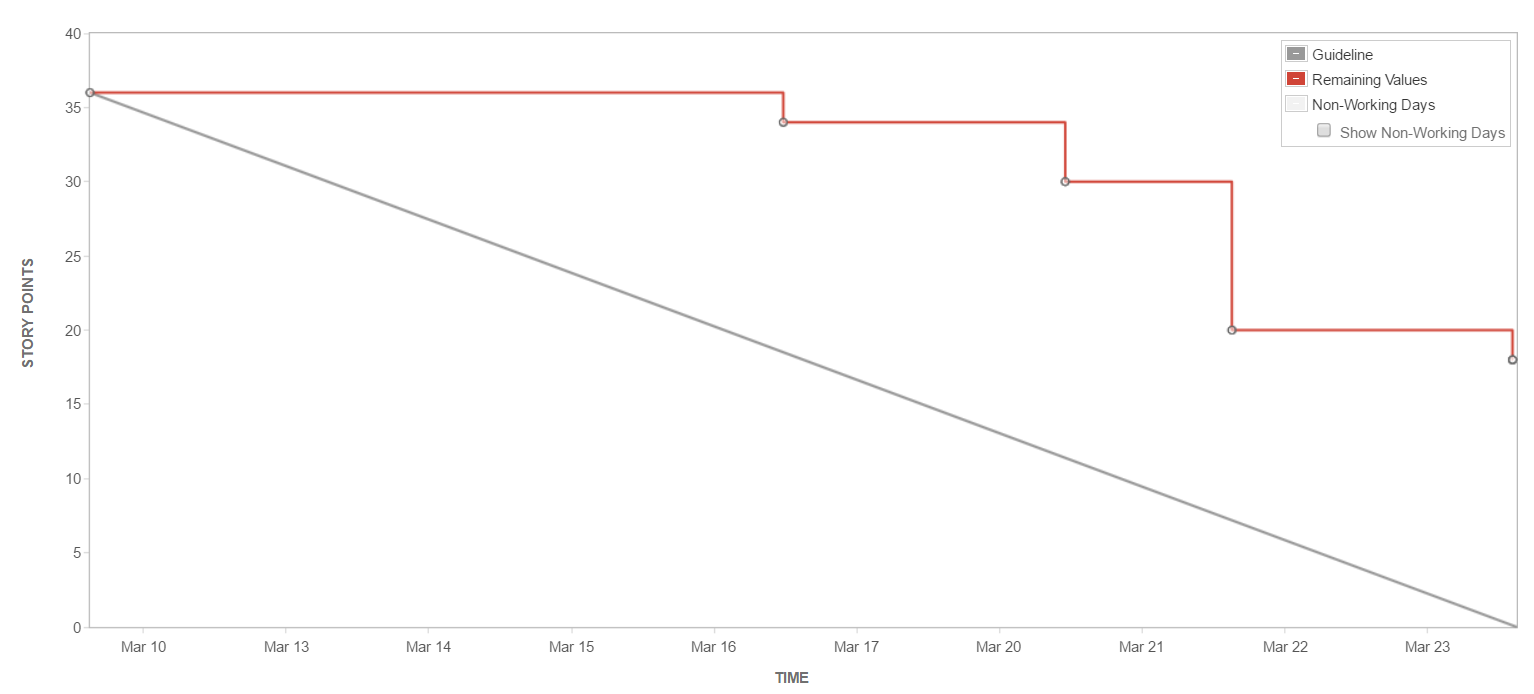
\includegraphics[width=\textwidth]{images/DOCKLSprint4}
    \caption[Burndown chart from the 4th sprint]{The burndown chart for the 4th sprint shows how sprints generally progressed on average throughout the project.}
    \label{fig:burndownChart}
\end{figure}

We will take a brief look at Figure~\ref{fig:burndownChart} which illustrates the burndown chart of the 4th sprint during development as it shows data that was fairly consistent throughout the other sprints. 

The first observation is that most issues generally were finished throughout the second week of the sprint rather than issues regularly finished as the guideline suggests. This is mostly due to the fact that the issues were rather large and not split up into subtasks very often. Doing so would better reflect project progress on Jira, but at the same time this would incur a fair amount of additional overhead per sprint by having to set up subtasks per issue. 

The next apparent observation is overscope. Most of the sprints after sprint 1 ended up having some overscope. The overscope was mostly related to being able to finish a docking kit while also working on other functionality of the game at the same time. This could certainly have been improved by looking at the statistics of previous sprints and manage expectations accordingly. The estimations for some of the game functionalities ended up being estimated for lower story point values than they required due to unexpected issues and bugs which resulted in a lack of resources needed to finish some of the docking kits for the sprint. 

In relation to actually working on docking kits, fortnightly sprints ended up fitting well. Designing and implementing the base functionality of most kits required one week of time while the other week was spent on bug fixing and polish. 

Working with Jira allowed us to setup sprints and issues in a tidy manner, but had a lot of additional functionality we never used although we can imagine a lot of it being useful for managing larger teams. 

Despite there having been some overscope during development, using Scrum allowed us to continue developing new increments without necessarily cutting or rushing core functionality of the game due to direct deadlines. The benefit of also having a rather relaxed scope for the game was that it meshed well with Scrum and agile development in general. 